\documentclass[aspectratio=169]{beamer}
\usepackage[utf8]{inputenc}               % codificacao de caracteres
\usepackage[T1]{fontenc}                  % codificacao de fontes
\usepackage[english,brazilian]{babel}     % idioma
\usetheme{Madrid}                         % tema
% \usecolortheme{orchid}                  % cores
\usefonttheme[onlymath]{serif}            % fonte modo matematico
% \usepackage[authoryear,round,longnamesfirst]{natbib}
\usepackage{graphicx}
% Pacote para escrever algorítmos no Latex
\usepackage[ruled,vlined]{algorithm2e}
\usepackage{lmodern}
\usepackage{array}
\usepackage{multirow}
\usepackage{booktabs}


% Titulo
\title[\sc{Três Ensaios em Comportamentos dos Preços}]{Três Ensaios em Comportamento dos Preços na Economia Brasileira}
\author{Hudson Chaves Costa}
\institute{PPGE - UFRGS} 
\date{\today}


\usepackage{Sweave}
\begin{document}
\Sconcordance{concordance:apresentacao.tex:apresentacao.Rnw:%
1 24 1 1 0 444 1}



\begin{frame}
  \titlepage
Orientador: Prof. Dr. Sabino Porto da Silva Júnior
\end{frame}

\begin{frame}[plain]\frametitle{Sumário}
\small\tableofcontents
\end{frame}

\section{Ensaio 1}
  
\begin{frame}\frametitle{}
	\begin{center}
	{\Huge Ensaio 1}
	\end{center}
\end{frame}

\subsection{Introdução/Motivação}

\begin{frame}\frametitle{Introdução/Motivação}
  \begin{itemize}
  \item Firmas individuais não ajustam seus preços em contrapartida de choques relevantes na economia:
    \begin{itemize}
    \item Hipótese em modelagem macroeconômica;
    \end{itemize}
  \item Comportamento microeconômicos de determinação de preços adotado pelos agentes:
    \begin{itemize}
    \item Tempo-Dependente;
    \item Estado-Dependente.
    \end{itemize}
  \item Bancos Centrais têm usado a política de metas de inflação:
    \begin{itemize}
    \item Meta definida em termos de um índice de preços agregado;
    \item Rigidez x Flexibilidade nos preços.
    \end{itemize}
  \item A partir disso, foi natural o surgimento de pesquisas com o objetivo de diferir a análise empírica da rigidez nominal dos preços baseada em dados agregados da avaliação do comportamento dos preços por meio de microfundamentos.
  \end{itemize}
\end{frame}

\subsubsection{Justificativa}

\begin{frame}\frametitle{Introdução/Motivação}
\textbf{Justificativa}
\begin{itemize}
% \item Em particular, \citet{bils2004some,nakamura2008five,klenow2008state,dhyne2006price,gouvea2007nominal,matos2009comportamento,lopes2008rigidez,bunn2012examining}.
\item A dinâmica do comportamento dos preços individuais proporciona vários desdobramentos que são bastantes debatidos na literatura dado o impacto que podem causar;
  \begin{itemize}
  \item A sua não compreensão levou a distintas abordagens para a análise da velocidade e intensidade de transmissão da política monetária
  \end{itemize}
\item A falta de estudos que gerassem empiricamente um diagnóstico da definição e grau de rigidez de preços individuais;
\item Limitação de acesso a base de dados
\end{itemize}
\end{frame}

\subsubsection{Objetivos}

\begin{frame}\frametitle{Introdução/Motivação}
\textbf{Objetivos}
\begin{itemize}
\item Avaliar empiricamente a rigidez nominal dos preços na economia brasileira por meio de dados coletados da \emph{web}
\item Propor um índice de inflação oriundo da mesma fonte de dados;
\item Questinamentos:
  \begin{itemize}
  \item É possível utilizar os dados coletados da internet como \emph{proxy} para a inflação divulgada pelos órgãos públicos?
  \item Quão frequentemente os preços se alteram?
  \item Existe heterogeneidade da rigidez nominal entre setores?
  \item A probabilidade de mudança dos preços pode variar ao longo da duração dos preços?
  \item Quais são as variáveis condicionantes para o risco de alteração nos preços?
  \end{itemize}
\end{itemize}
\end{frame}

\subsection{Referencial Bibliográfico}

\begin{frame}\frametitle{Referencial Bibliográfico}
  \begin{itemize}[<+->]
  \item Modelos de Precificação
    \begin{itemize}
      \item Contratos de Calvo/Taylor
      \item Custo de Menu
      \item Informação Rígida
      \item Ira do Cliente
    \end{itemize}
  \item Preços Rígidos e Preços Flexíveis
  \item Modelos Tempo-Dependente e Estado-Dependente
  \item Estudos Empíricos
  \end{itemize}
\end{frame}

\begin{frame}\frametitle{Referencial Bibliográfico - Modelos de Precificação}
  \textbf{Contratos de Calvo/Taylor}
  \begin{itemize}
  \item No modelo de Calvo (1983) a probabilidade de um preço mudar é constante:
    \begin{itemize}
      \item Independe da última vez que uma firma mudou seu preço;
      \item Função risco constante.
    \end{itemize}
  \item Taylor (1980) define que os preços nominais são fixos por um certo número de períodos:
    \begin{itemize}
      \item Os preços são fixos por N períodos;
      \item Taxa de risco é zero para todas as durações exceto N.
    \end{itemize}
  \item Generalização dos modelos de Taylor e Calvo:
    \begin{itemize}
      \item Em Taylor, existem muitos setores com diferentes tamanhos de preços e dentro de cada setor há um processo de Taylor simples;
      \item Em Calvo, a estratégia de definição dos preços considera múltiplos setores.
    \end{itemize}
  \end{itemize}
\end{frame}

\begin{frame}\frametitle{Referencial Bibliográfico - Modelos de Precificação}
  \textbf{Custo de Menu}
  \begin{itemize}
  \item Assume que a mudança no preço é custosa e isto impede que as firmas alterem seus preços continuamente;
  \item Os modelos usualmente são resolvidos usando métodos numéricos e assim, não há expressão analítica para a taxa de risco.
  \end{itemize}
  \textbf{Ira do Cliente}
  \begin{itemize}
  \item Modelo de Rotemberg (2005) salienta que os clientes sempre analisam as decisões de precificação das firmas;
  \item Percepção de justiça;
  \item Firmas podem abandonar alterações nos preços para evitar a ira do cliente;
  \item Em rápido crescimento da inflação os clietnes aceitam os ajustes dos preços;
  \item Empresas podem alterar seus preços dentro de um calendário de forma que os clientes desenvolvam suas crenças.
  \end{itemize}
\end{frame}

\begin{frame}\frametitle{Referencial Bibliográfico - Modelos de Precificação}
  \textbf{Informação Rígida}
  \begin{itemize}
  \item Firmas sofrem com o custo de coletar informações sobre as condições econômicas e concorrentes;
  \item Em cada período, a partir de novas informações, define-se um novo padrão de preços ótimos;
  \item Todas as firmas mudam seus preços em todo o tempo em modelos de rigidez de informação;
  \item Contudo, é contraditório nas evidências empíricas baseadas em dados individuais;
  \item Estudos combinaram este modelo com custo de menu (Klenov e Willis, 2007;II e Edward, 2010)
  \item \textbf{Solução:} Pagar custos ou aprender com as ações das outras empresas.
  \end{itemize}
\end{frame}

\begin{frame}\frametitle{Referencial Bibliográfico - Preços Rígidos e Preços Flexíveis}
  \begin{itemize}
  \item A alternativa aos modelos de preços rígidos é o modelo de \textbf{Lucas (1972)} onde os preços são flexíveis e a imperfeição nominal é informacional;
    \begin{itemize}
    \item Produtor observa uma mudança no preço do seu produto e não sabe distinguir se isso é resultado de alterações no preço relativo ou nível agregado de preços;
    \item A partir de uma expansão monetária não-observada, o melhor que cada produtor pode fazer é admitir que uma parte do aumento da demanda por seu produto reflete um choque de preços relativos;
    \item \textbf{Consequência:} Expansão monetária tem efeitos reais e não apenas nominais sobre os preços.
    \end{itemize}
  \end{itemize}
\end{frame}

\begin{frame}\frametitle{Referencial Bibliográfico - Preços Rígidos e Preços Flexíveis}
  \begin{itemize}
  \item A vertente \textbf{novo-keynesiana} estabelece a hipótese de existência de rigidez nominal tanto nos preços quanto nos salários;
  \item Essas variáveis nominais têm dificultade de ajuste e provocam impactos reais sobre o produto;
  \item \textbf{Consequência:} Expansão monetária pode causar diferentes impactos sobre cada preço da economia dependendo do grau de rigidez nominal de cada bem;
  \item \textbf{Consequência:} Se a rigidez for diversificada, resultará em alterações nos preços relativos provocando impactos reais
  \end{itemize}
\end{frame}

\begin{frame}\frametitle{Referencial Bibliográfico - Modelos Tempo-Dependente e Estado-Dependente}
\textbf{Tempo-Dependente}
  \begin{itemize}
  \item A probabilidade dos preços mudarem depende apenas do período pelo qual o preço está fixo;
  \item Função risco tem um forma constante em relação à duração dos preços
  \item Calvo (1983) assume uma função risco plana:
    \begin{itemize}
    \item Oportunidade de alterar os preços com uma probabilidade constante em cada período;
    \item Curva de Phillips Novo-Keynesiana é derivada do modelo de Calvo com competição monopolística.
    \end{itemize}
  \item Taylor (1980) tem uma função risco constante:
    \begin{itemize}
    \item Preços mudam no começo do contrato e não se alterarm dentro do período de durabilidade;
    \item Taxa de risco toma o valor da unidade no começo do contrato e 0, por conseguinte. 
    \end{itemize}
  \end{itemize}
\end{frame}

\begin{frame}\frametitle{Referencial Bibliográfico - Modelos Tempo-Dependente e Estado-Dependente}
\textbf{Estado-Dependente}
  \begin{itemize}
  \item Custo de Menu de Barro (1972) e Sheshinski e Weiss (1977);
  \item Tendem a ter maior fundamentação microeconômica;
  \item Probabilidade condicional do preço alterar depende das variáveis de estado, preços relativos e taxas de inflação;
  \item Função risco pode mudar sua forma em resposta à choques reais ou monetários em transição;
    \begin{itemize}
    \item Forma constante em \emph{steady state}
    \end{itemize}
  \end{itemize}
\end{frame}

\begin{frame}\frametitle{Referencial Bibliográfico - Estudos Empíricos}
  \begin{itemize}
  \item Trabalhos utilizando microdados para analisar a rigidez nominal nos preços;
  \item Viabilidade de avaliação da rigidez em vários níveis (setores, cidades, cesta de consumo, ...);
  \item \textbf{Bils e Kenow (2004)}:
    \begin{itemize}
    \item Alterações nos preços mensais de 350 produtos e serviços que representavam em torno de 70\% da cesta de consumo do CPI no período de 1995 a 1997 nos EUA;
    \item \textbf{Conclusão:} Os preços se alteravam tipicamente em torno de uma vez por ano
    \end{itemize}
  \end{itemize}
\end{frame}

\begin{frame}\frametitle{Referencial Bibliográfico - Estudos Empíricos}
  \begin{itemize}
  \item \textbf{Nakamura e Steinsson (2008)}:
    \begin{itemize}
    \item Avaliaram os preços mensais de 270 produtos que representavam 70\% da cesta de consumo do CPI no período de 1998 a 2005 para os EUA;
    \item \textbf{Conclusões:} 
      \begin{itemize}
      \item Um terço das alterações nos preços são em relação a quedas;
      \item A frequência de aumento nos preços está fortemente relacionada com a inflação enquanto a queda não;
      \item A frequência das alterações nos preços é altamente sazonal;
      \item Função risco com inclinação ascendente para produtos individuais
      \end{itemize}
    \end{itemize}
  \end{itemize}
\end{frame}

\begin{frame}\frametitle{Referencial Bibliográfico - Estudos Empíricos}
  \begin{itemize}
  \item \textbf{Lopes (2008)}:
    \begin{itemize}
    \item Analisaram mais de 6 milhões de preços do índice de preços ao consumidor da FIPE
    \item \textbf{Conclusões:} 
      \begin{itemize}
      \item A frequência média de mudança nos preços é de 32,35\% ao mês;
      \item Os preços duram em média 2,5 meses;
      \item Há grande heterogeneidade entre produtos quanto ao comportamento dos preços;
      \item 40\% das mudanças são para baixo;
      \item As funções de risco são decrescentes 
      \end{itemize}
    \end{itemize}
  \end{itemize}
\end{frame}

\subsection{Metodologia}

\begin{frame}\frametitle{Metodologia}
  \textbf{Web Scraping}
  \begin{itemize}
  \item Envolve escrever algoritmos que executam automaticamente o que nós fazemos manualmente quando navegamos por uma página;
  \item É o processo de tirar informações desestruturadas de páginas da web e transformá-las em informações estruturadas;
  \item As páginas são escritas em \emph{Hyper Text Markup Language}(HTML) e possuem \emph{tags} que permitem localizar e navegar dentro do código;
  \item Através de um coletor é possível arquiteturar e executar de forma lógica e escalável todo esse processo
  \end{itemize}
\end{frame}

\begin{frame}\frametitle{Metodologia}
  \begin{figure}[hb]
  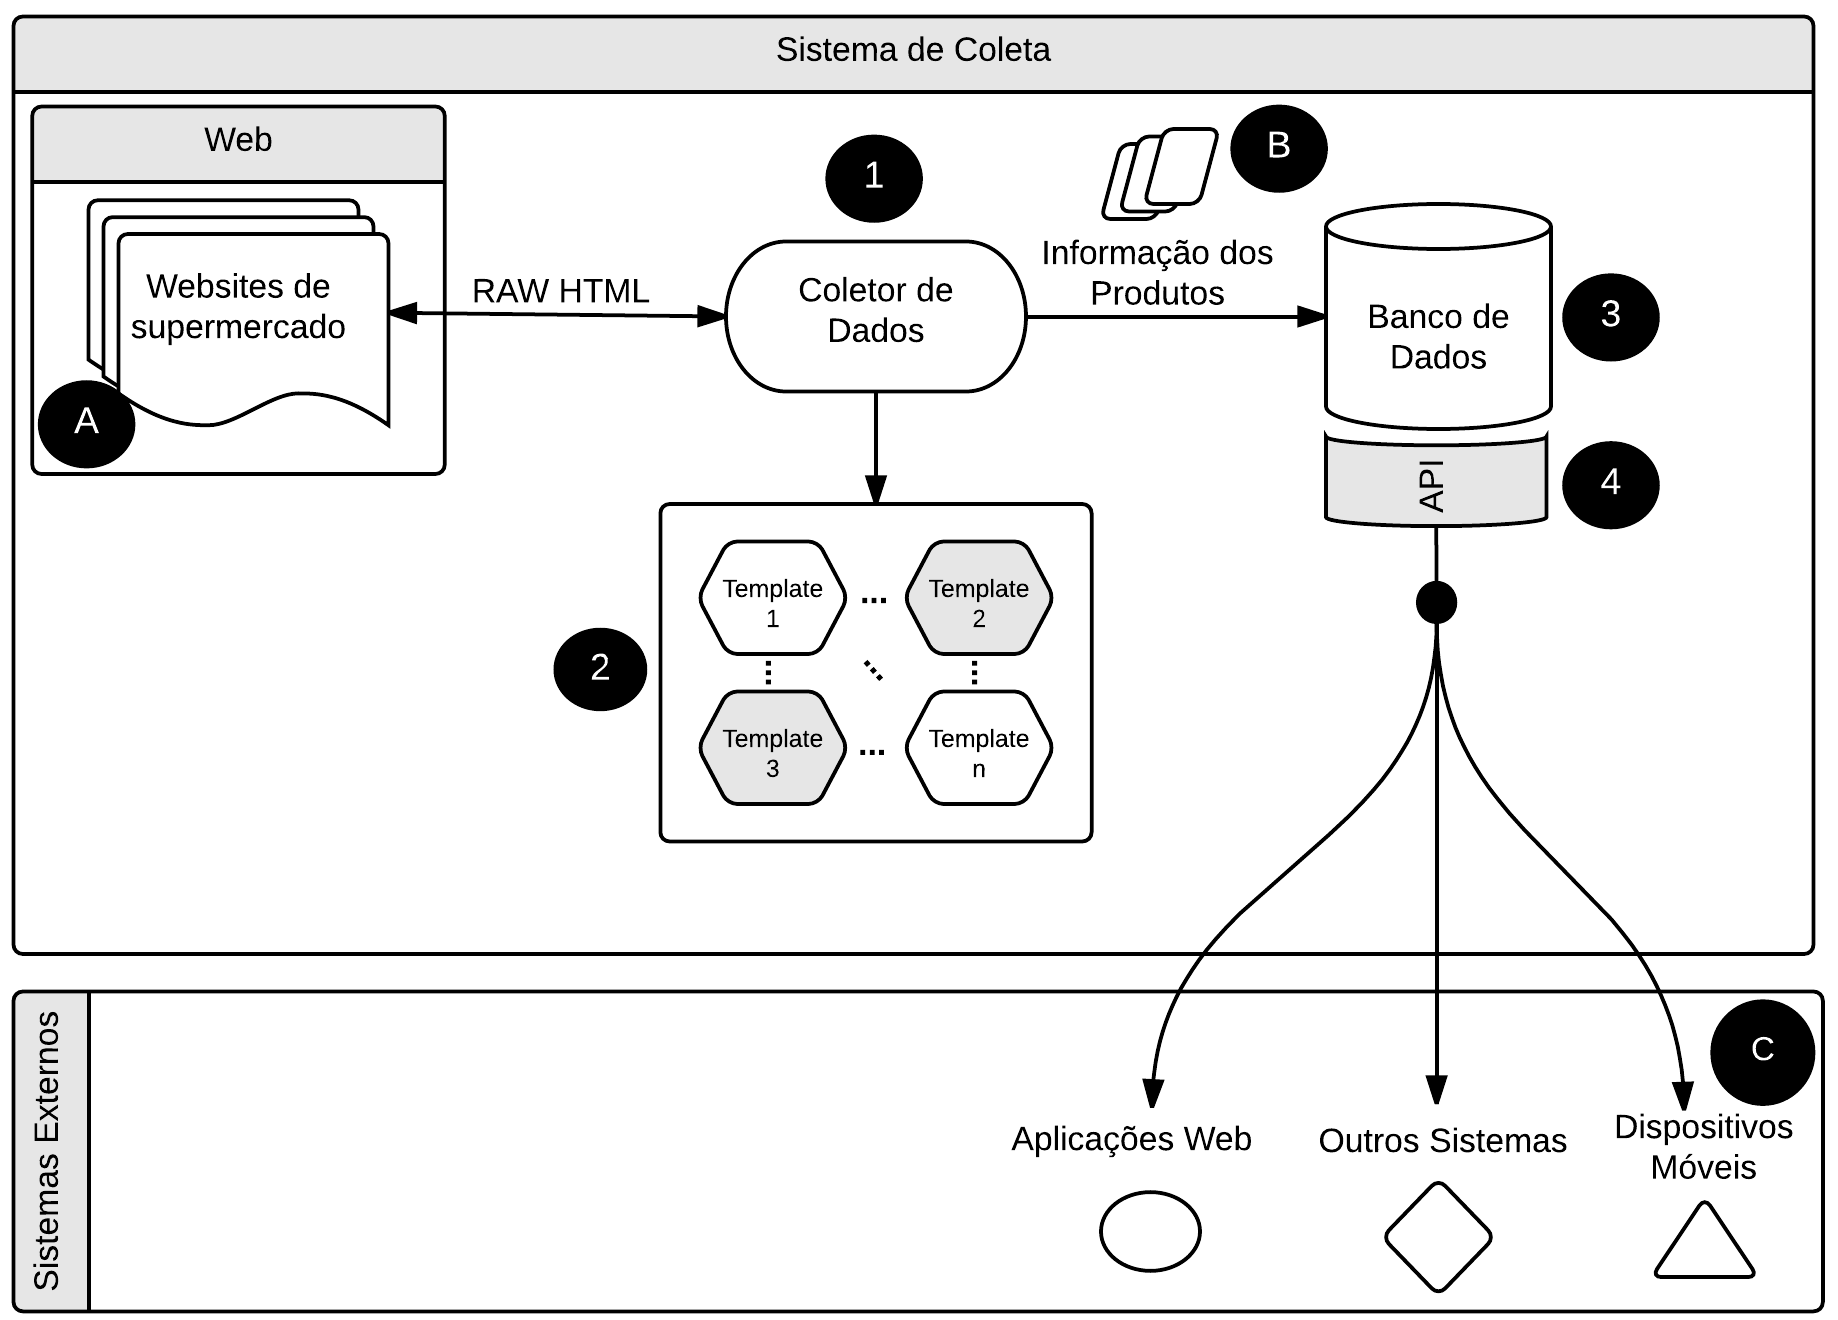
\includegraphics[width=3in]{WebScraping.png}
  \label{fig01en01}
  \caption{Arquitetura do Sistema de Coleta e Disponibilização dos Dados}
  \end{figure}
\end{frame}

\begin{frame}
\begin{centering}
\scalebox{0.95}{%
\begin{algorithm}[H]
 \Dados{T $\leftarrow$ (t)${^N_{i=1}}$; tal que T é uma lista de templates}
 \Resultado{Armazenados produtos estruturados em um banco NoSQL}
 \BlankLine
 \SetKwFunction{conectarNoSQL}{conectarNoSQL}
 \SetKwFunction{visitarWebsite}{visitarWebsite}
 \SetKwFunction{extrairInfo}{extrairInfo}
 \SetKwFunction{estruturarProduto}{estruturarProduto}
 \SetKwFunction{armazenarEmNoSQL}{armazenarEmNoSQL}
 \emph{Inicialização:} nosql $\leftarrow$ \conectarNoSQL{url, porta, ...}\;
 \BlankLine
 \For{(t, u) \textbf{in} T}{
   rawHtml $\leftarrow$ \visitarWebsite{u}\;
   P $\leftarrow$ \extrairInfo{rawHtml, t}\;
 	\For{p \textbf{in} P}{
 	ps $\leftarrow$ \estruturarProduto{p}\;
 	nosql.\armazenarEmNoSQL{ps}\;
 	}
 }
 \caption{Algoritmo para coleta de dados.}
\end{algorithm}}
\end{centering}
\end{frame}

\begin{frame}\frametitle{Metodologia}
  \textbf{Índice de Preços Online}
  \begin{itemize}
  \item Combina dados coletados com as estruturas de ponderação oficiais do IBGE para as categorias de cestas de mercadorias de cada índice de inflação;
  \item Dados diários serão utilizados para construir o índice de preços online o que é útil para observar padrões de curto prazo;
  \item Utiliza os preços de todos os produtos disponíveis para compra em cada site:
    \begin{itemize}
    \item A cesta de bens muda dinamicamente ao longo do tempo;
    \item Número de preços por produto tende a ser maior do que os coletados usualmente;
    \end{itemize}
  \end{itemize}
\end{frame}

\begin{frame}\frametitle{Metodologia}
  \textbf{Índice de Preços Online}
  \begin{itemize}
  \item As mudanças de preço são calculadas em nível de produto, então as médias dentro das categorias usando média geométrica ponderada e finalmente agregando entre as categorias com uma média aritmética ponderada. 
  \end{itemize}
  \begin{exampleblock}{Média Geométrica na Categoria}
  \[
  R_{t,t-1}^{j}=\prod_{i}(\frac{p_{t}^{i}}{p_{t-1}^{i}})^{\frac{1}{n_{j,t}}}
  \]
  \end{exampleblock}
onde $p_{t}^{i}$ é o preço do bem $i$ no tempo $t$, ${n_{j,t}}$ é o número de produtos na categoria $j$ que estão presentes na amostra neste dia
\end{frame}

\begin{frame}\frametitle{Metodologia}
  \textbf{Índice de Preços Online}
  \begin{exampleblock}{Índice em nível de Categoria}
  \[
  I_{t}^{j}=R_{1,0}^{j}\ast{R}_{2,1}^{j}\ast{...}\ast{R}_{t,t-1}^{j}
  \]
  \end{exampleblock}
onde $I_{t}^{j}$ é o índice da categoria $j$ considerando as médias até o mês anterior.
 \begin{exampleblock}{Índice de Preços}
  \[
  IPO_{t}=\sum_{j}{\frac{w_{j}}{w}I_{t}^{j}} 
  \]
  \end{exampleblock}
onde $w_{j}$ é o peso oficial utilizado pelo IBGE e ${w}$ a soma dos pesos. 
\end{frame}

\begin{frame}\frametitle{Metodologia}
  \textbf{Rigidez de Preços}
  \begin{itemize}
  \item Diversas estatísticas poderão ser utilizadas para avaliar a rigidez de preços:
    \begin{itemize}
    \item Frequência de produtos com alterações diárias;
    \item Frequência de alta e baixa em relação ao total de alterações nos preços em um dia;
    \item Tamanho da mudança nos preços por meio do valor absoluto das alterações;
    \item Avaliação da distribuição dos tamanhos (bimodal, assimetria).
    \end{itemize}
  \item Todas essas estatísticas refletem a \textbf{probabilidade incondicional}
  \end{itemize}
\end{frame}

\begin{frame}\frametitle{Metodologia}
  \textbf{Análise de Sobrevida}
  \begin{itemize}
  \item Em análise de sobrevivência a variável resposta é o tempo até a ocorrência de um evento de interesse (tempo de falha);
  \item No contexto de preços, estamos interessados no tempo até o ajuste do preço;
  \item Assim, tanto o aparecimento do risco e o evento de falha ocorrem quando uma firma muda seus preços;
  \item Função de sobrevivência:
    \begin{itemize}
    \item Probabilidade de uma observação sobreviver (preço não se alterar) ao tempo $t$;
    \end{itemize}
  \item Função Risco:
  \begin{itemize}
    \item Probabilidade limite de que a mudança no preço ocorra em $t$, condicional ao preço não se alterar até este momento;
    \item Mede o risco instantâneio de um preço se alterar
    \end{itemize}
  \end{itemize}
\end{frame}

\begin{frame}\frametitle{Metodologia}
  \textbf{Análise de Sobrevida}
  \begin{exampleblock}{Risco}
  \[
  h(t)=\lim_{\Delta t\rightarrow 0}{\frac{Pr(t<T<t+\Delta t|t<T)}{\Delta t}=\frac{f(t)}{1-F(t)}} 
  \]
  \end{exampleblock}
onde $T$ é a variável aleatória que mede a duração do preço, com função densidade $f(t)$ e densidade acumulada $F(t)$ e $h(t)$ o risco condicional ao preço não se alterar até este momento. 
  \begin{exampleblock}{Função Risco Suavizada}
  \[
\hat{h}\left(t \right)=\frac{1}{b}\sum_{j\epsilon D}{K}\left(\frac{t-{t}_{j}}{b}\right)\Delta \hat {H}\left({t}_{j}\right) 
  \]
  \end{exampleblock}
onde $K$ é um kernel com densidade simétrica, $b$ a \emph{bandwidth} de suavização e $D$ é o conjunto de vezes com mudanças nos preços.
\end{frame}

\begin{frame}\frametitle{Metodologia}
Para modelar a probabilidade de um preço mudar será preciso focar sobre os eventos de mudança nos preços. Assim, defina a variável $Y_{jkt}$:
  \begin{exampleblock}{Variável Binária}
  \[
Y_{jkt} =\begin{cases}1 &  P_{jkt} \neq P_{jk,t-1}\\0 & P_{jkt} = P_{jk,t-1}\end{cases}
  \]
  \end{exampleblock}
onde ${Y}_{jkt}$ indica se o preço do produto $j$ vendido pela firma $k$ foi alterado no começo do período $t$, e ${P}_{jk,t-1}$ é o preço do produto $j$ vendido pela firma $k$ no período $t$.

A escolha das variáveis explicativas para o modelo dependerá do mecanismo de formação de preços subjacente. Se assumimos Calvo (1983):

  \begin{equation}
  Pr({Y}_{jkt}=1)=\frac{exp({\beta}_{0})}{1+exp({\beta}_{0})} 
  \end{equation}
\end{frame}

\begin{frame}\frametitle{Metodologia}
  \textbf{Determinantes para a probabilidade do preço alterar}
  \begin{itemize}
  \item Inflação;
  \item Tempo desde a última alteração;
  \item Tamanho da alteração anterior;
  \item Variável de demanda: montante de vendas, por exemplo. Será preciso definir uma variável que represente a demanda dos produtos;
  \item Atratividade dos preços: preços finalizando com os dígitos 9, 5 ou 0;
  \item Efeito sazonal e anual;
  \item Variáveis setoriais.
  \end{itemize}
\end{frame}

\begin{frame}\frametitle{Metodologia}
Assim, a representação do modelo logit será:
  \begin{exampleblock}{Modelo Logit}
  \[
Pr\left( { Y }_{ jkt }=1 \right) =\frac { exp\left( { X }_{ jkt }\beta +{ u }_{ jk }+{ \varepsilon  }_{ jkt } \right)  }{ 1+exp\left( { X }_{ jkt }\beta +{ u }_{ jk }+{ \varepsilon  }_{ jkt } \right)  }
  \]
  \end{exampleblock}
onde ${ X }_{ jkt }$ é um vetor linha de variáveis exógenas, $\beta$ é um vetor coluna dos coeficientes do modelo logit e ${ \varepsilon  }_{ jkt }$ é um termo de erro. Por fim, pode-se distinguir a variável $Y_{jkt}$ entre alterações em todos os preços ou excluir as promoções da análise.
\end{frame}

\subsection{Cronograma}

\begin{frame}\frametitle{Cronograma}
\begin{table}[h]
\begin{tabular}{llllll}
\hline
\multicolumn{1}{c}{\textbf{Atividades}} & 2015/01               & 2015/02               & 2015/03               & 2015/04               & 2016/01               \\ \hline
Pesquisa Bibliográfica                  & \multicolumn{1}{c}{X} & \multicolumn{1}{c}{X} &                       &                       &                       \\
Mapeamento de sites                     & \multicolumn{1}{c}{X} &                       &                       &                       &                       \\
Implementação do sistema de coleta      & \multicolumn{1}{c}{X} &                       &                       &                       &                       \\
Criação dos Índices de Inflação         &                       & \multicolumn{1}{c}{X} &                       &                       &                       \\
Análise de Rigidez                      &                       &                       & \multicolumn{1}{c}{X} &                       &                       \\
Determinantes da Inflação nas Regiões   &                       &                       &                       & \multicolumn{1}{c}{X} &                       \\
Redação Final da Tese                   &                       &                       &                       & \multicolumn{1}{c}{X} & \multicolumn{1}{c}{X} \\
Entrega da Tese para Defesa             &                       &                       &                       &                       & \multicolumn{1}{c}{X} \\ \hline
\end{tabular}
\end{table}
\end{frame}


\end{document}


% %%%%%%% REFERÊNCIAL BIBLIOGRÁFICO
% 
% \section{REFERÊNCIAS}
% \begin{frame}{Bibliography}
% \bibliographystyle{apalike}
% \bibliography{geral}
 
\end{document}
